% (c) GreenSocs Ltd
% author: Christian Schroeder <schroeder@eis.cs.tu-bs.de>

%\documentclass[a4paper,12pt]{scrartcl}
\documentclass[a4paper,12pt,oneside]{gsbook}

\usepackage[utf8]{inputenc}

\usepackage{helvet}

\usepackage{hyperref}

\usepackage{greensocs}

\usepackage{graphicx}

\usepackage{multicol}

\usepackage{fancyhdr}

\usepackage{multirow}

\usepackage{tabularx}

\usepackage[dvips]{rotating} 

%% Christian's package CS_inputs
%\usepackage{verbatimfiles}
%\usepackage[outline,light]{draftcopy}

%\usepackage{ngerman}					% Regeln und Definitionen fuer deutschen Sprachraum
%\usepackage[latin1]{inputenc} % Umlaute
%\usepackage[T1]{fontenc}      % Woerter mit Umlauten richtig trennen
%\usepackage{ae}%um Einbindung von Type1-Fonts in PDF zu ermoeglichen
\usepackage{amsmath}						% Mathematik, fuer \text innerhalb $ $
%\usepackage[pdftex]{graphicx}
\usepackage{pifont} % needed for \ding{110} etc. (see new items)

\usepackage{lscape}			% ermoeglicht Querformat-Seiten, zwischen \begin{landscape} \end{landscape}

\usepackage{enumerate}	% ermoeglicht enumerate-Umgebung mit Option zu veraendern

\usepackage{listings}   % Listing von Programmcode
\lstloadlanguages{C}		% laedt die Regeln fuer Programmiersprache C
\usepackage{marvosym}		% fuer \lstset prebreak={\Righttorque} (Pfeil beim Umbruch einer Zeile)
\lstset{% general command to set parameter(s)
	basicstyle=\normalsize\ttfamily, % print whole listing
	stringstyle=\ttfamily, % typewriter type for strings
	keywordstyle=\ttfamily,
	showstringspaces=false,
	language=C,
	breaklines=true
}
\usepackage{color}			% fuer die Farbe der comments
\definecolor{keywordblue}{RGB}{0,0,255}
\definecolor{commentgreen}{RGB}{0,128,0}

\usepackage{float}
\restylefloat{table} % sorgt dafuer, dass [H] dafuer sorgt, dass Tabelle GENAU da ist, wo sie steht
\restylefloat{figure} % sorgt dafuer, dass [H] dafuer sorgt, dass figure GENAU da ist, wo sie steht
\usepackage{array}   % ermoeglicht komplexere Tabellen, vor allem mit automatischem Umbruch innerhalb der Zellen

%\usepackage{scrpage2} % ermoeglicht eigene Kopf- und Fu�zeilen, gehoert zum KOMA
%\usepackage{thumbindices} %create chapter thumb index on outer right side of pages (only works correct for pdfs)
%\usepackage{chapterthumb}
%create chapter thumb index on outer right side of pages (only works correct for pdfs)
%\usepackage{thumb}
\usepackage{longtable}
\usepackage{multirow}

\usepackage{xspace}
\usepackage{fancybox}  % Schattierte oder sonstig besondere Rahmen
\definecolor{dunkelgrau}{gray}{0.55}
\definecolor{hellgrau}{gray}{0.9}
\definecolor{hellhellgrau}{gray}{0.92}
\definecolor{weiss}{gray}{1}
\definecolor{schwarz}{gray}{0}
\usepackage{hhline}
\usepackage{colortbl}  % ermoeglicht farbige Tabellen

% aus de-tex-faq 5.3.4
% verhindert Hurenkinder und Schusterjungen (einzelne Zeilen nach/vor Seitenumbruch)
%\clubpenalty = 10000                               % TODO: wohlueberlegt einsetzen!!
%\widowpenalty = 10000 \displaywidowpenalty = 10000 % TODO: wohlueberlegt einsetzen!!

% EIGENE MAKROS:

% %%% ZwischenUberschrift %%%
\setlength{\fboxrule}{0.05cm}
%\newcommand{\ZwischenUberschrift}[1]{\vspace*{3ex}\textsf{\bfseries{#1}}\\[2ex]}
\newcommand{\ZwischenUberschrift}[1]{\vspace*{3ex}
	\noindent % nicht einruecken
	\boxput{
		\makebox(0,0)
			{
				\fcolorbox{weiss}{hellgrau}{\parbox[b]{\textwidth}{~}}
			}
	}
	{\parbox[b]{\textwidth}{\hspace*{2em}\textsf{\bfseries{#1}}}
	{	}
	}\vspace*{1ex}
	\nopagebreak
}

% %%% Verzeichnis %%%
\newsavebox{\VerzeichnisBox}
\newcommand{\Verzeichnis}[1]
	{
			\savebox{\VerzeichnisBox}{
\includegraphics{csimages/verzeichnis.eps} \textsf{#1}}
			\usebox{\VerzeichnisBox}
	}
	
% %%% Datei %%%
\newsavebox{\DateiBox}
\newcommand{\Datei}[1]
	{
			\savebox{\DateiBox}{
\includegraphics{csimages/datei.eps} \textsf{#1}}
			\usebox{\DateiBox}
	}
\newcommand{\DateiNoImg}[1]
	{
			\textsf{#1}
	}

% %%% Menue %%%
\newcommand{\Menue}[1]{\textsc{#1}}
% %%% Button %%%
\newcommand{\Button}[1]{\textsc{#1}}
% %%% Eingabe %%%
\newcommand{\Eingabe}[1]{
	\fcolorbox{weiss}{schwarz}{\textcolor{weiss}{\ttfamily #1}}
}

\newcommand{\befehl}[1]{\protect\mbox{\textsf{\textbf{\footnotesize{#1}}}}}			% einheitliche Befehle meines Protokolls
\newcommand{\Ohm}{$ \Omega $\xspace}										% Ohm fuer die Stueckliste
\newcommand{\uF}{$ \mu \text{F} $\xspace}
\setlength{\fboxrule}{0.05cm} % Rahmenbreite fuer box
\newcommand{\Achtung}[1]{	
	\begin{samepage}
		\noindent % nicht einruecken
		\fcolorbox{dunkelgrau}{hellhellgrau}{\parbox[b]{12cm}{#1}}
	\end{samepage}
}
\newcommand{\Parameter}[1]{\textsc{#1}} % Fuers Protokoll

\renewcommand{\labelitemi}{\textcolor{dunkelgrau}{\ding{110}}} % neues Zeichen fuer Aufzaehlunsebene 1
\renewcommand{\labelitemii}{\textcolor{dunkelgrau}{\ding{108}}} % neues Zeichen fuer Aufzaehlunsebene 2
\renewcommand{\labelitemiii}{\textcolor{dunkelgrau}{$\bullet$}} % neues Zeichen fuer Aufzaehlunsebene 2

\usepackage{makeidx}

\makeindex % ermoeglicht das erzeugen von Idizes mit \index{eintrag} Dann mit Makeindex weiterverarbeiten

\newcommand{\Note}[3]{
	\vspace{.5cm}
	\begin{minipage}{15cm}
		\noindent % nicht einruecken
		\rule{\textwidth}{.3pt}
		\Datei{} \textbf{\textsf{#1}}
		
		\textbf{#2}		
		
		#3
		
		\noindent % nicht einruecken
		\rule{\textwidth}{.3pt}
	\end{minipage}
	\vspace{.5cm}
}

% %%% Warning %%%
\newsavebox{\WarningSymbolBox}
\newcommand{\WarningSymbol}[1]
	{
			\savebox{\WarningSymbolBox}{
\includegraphics[height=1.7ex]{csimages/warning.eps} #1}
			\usebox{\WarningSymbolBox}
	}


%\usepackage{xspace}

% Fuer \begin{landscape}
\usepackage{lscape}

% allows [H] in figure
\usepackage{float}
\restylefloat{figure}

%Includes fuer mathematische Formeln
\usepackage{amsmath,amsthm,latexsym}
\usepackage{wasysym}

\sloppy % Verhindert uebervolle H-Boxen (aber groessere Spaces!)
\nonfrenchspacing % Abstand nach Satzende immer gleich gross

% Verhindern von Schusterjungen (club) und Hurenkindern (widow)
\clubpenalty=10000
\widowpenalty=10000
\displaywidowpenalty=10000 

% sets spacing between paragraphs
\parskip 7.2pt

% Farbe
\usepackage{color}  

% Symbole
\usepackage{marvosym} 

% Farbe fuer listings
\definecolor{stringblue}{RGB}{0,0,255}
\definecolor{keywordred}{RGB}{160,0,0}
\definecolor{commentgreen}{RGB}{0,128,0}
% Symbole fuer Listing-Umbruch-Pfeil
\newcommand{\linebreaksign}{\hbox{\space\Righttorque}} % marvosym S.28 symbols-letter.pdf
% Listings
\usepackage{listings}
\lstset{
  language=C++,
  %basicstyle=\ttfamily,
  breaklines=true,
  captionpos=b
  %breakatwhitespace=true% erlaubt line break nur bei einem whitespace
  aboveskip=15pt, % Abstand ueber einem Listing
  basicstyle=\ttfamily \small,
  %identifierstyle=\it,%\bf,
  commentstyle=\color{commentgreen} \ttfamily, % mach mich dunkler
  stringstyle=\color{stringblue} \ttfamily,
  keywordstyle=\color{keywordred},
  showstringspaces=false,
  numbers=left,
  numberstyle=\tiny,
  numberfirstline=true,
  firstnumber=1,
  stepnumber=5,
  numbersep=5pt,
  %prebreak=\mbox{\tiny$\linebreaksign$}, 
  prebreak=\Righttorque,
  frame=trbl, % Rahmen
  tabsize=2   % 2 spaces per tab
}

%\makeatletter
%\DeclareRobustCommand*\textsubscript[1]{%
%  \@textsubscript{\selectfont#1}}
%\def\@textsubscript#1{%
%  {\m@th\ensuremath{_{\mbox{\fontsize\sf@size\z@#1}}}}}
%\makeatother

\hypersetup{%
  plainpages=false,
  colorlinks,   % Ausschalten fuer Druckversion
  linkcolor=blue,
  bookmarksnumbered,
  pdftitle={GreenControl User's Guide},
  pdfsubject={User's Guide for the GreenSocs GreenControl Framework, GreenControl},
  pdfauthor={Christian Schroeder, Technical University of Braunschweig, Dept. E.I.S. and GreenSocs Ltd},
  pdfkeywords={SystemC GreenSocs GreenControl},
  pdfstartview=FitH
}
\author{Copyright GreenSocs Ltd 2007-2009\\ \\Developed by\\Christian Schr\"oder and Wolfgang Klingauf\\Technical University of Braunschweig, Dept. E.I.S.}
\title{GreenControl User's Guide\\(GreenControl v.3.0.0)}

\renewcommand{\theenumi}{\arabic{enumi}}
\renewcommand{\theenumii}{\arabic{enumi}.\arabic{enumii}}
\renewcommand{\theenumiii}{\arabic{enumi}.\arabic{enumii}.\arabic{enumiii}}
\renewcommand{\theenumiv}{\arabic{enumi}.\arabic{enumii}.\arabic{enumiii}.\arabic{enumiv}}

% with subsubsections in tableofcontents
\setcounter{secnumdepth}{3}
\setcounter{tocdepth}{3}


%% new commands for this document
\newcommand{\GreenBus}{\mbox{\textsc{\small GreenBus}}\xspace}
\newcommand{\GreenControl}{\mbox{\textsc{\small GreenControl}}\xspace}
\newcommand{\GreenConfig}{\mbox{\textsc{\small GreenConfig}}\xspace}
\newcommand{\GreenAV}{\mbox{\textsc{\small GreenAV}}\xspace}


\begin{document}

%Developed by Technical University of Braunschweig, Dept. E.I.S.
%Christian Schroeder
\maketitle

\tableofcontents

\listoffigures

% Chapter Introduction
% (c) GreenSocs Ltd
% author: Christian Schroeder <schroeder@eis.cs.tu-bs.de>

\chapter{GreenControl Introduction}

This section contains a brief overview of the implementation ideas for the {\em GreenControl} project. The \GreenControl framework is extendable with \textsl{plugins} which provide a service and add new functionality. See the project page\footnote{\GreenControl project page:  \href{http://www.greensocs.com/projects/GreenControl}{http://www.greensocs.com/projects/GreenControl}} for further documentation and downloads.

\section{Transaction-based approach}

The \GreenControl framework is based on a transaction-based approach. The \GreenControl Core is a router that connects user modules with service providers (plugins).
\begin{itemize}
	\item The connections are established via ports.
	\item Communication takes place using a special transaction container.
\end{itemize}

This concept is very similar to \GreenBus\footnote{\GreenBus project page: \href{http://www.greensocs.com/projects/GreenBus}{http://www.greensocs.com/projects/GreenBus}}.

\begin{figure}[htbp]
	\centerline{
		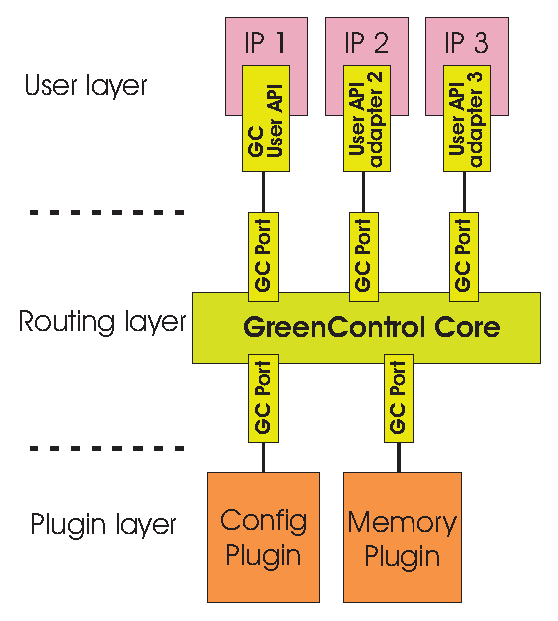
\includegraphics[width=10cm]{GreenControl.eps}} 
	\caption{GreenControl framework with service plugins.}
	\label{fig:GreenControl}
\end{figure}

Figure \ref{fig:GreenControl} shows the approach. The \GreenControl Core routes transactions between the IPs and plugins. One or more of the IPs may be a tool.



\section{Transaction container}
A transaction container contains generic attributes to transfer commands between the user modules and the service providers. The concepts of {\em atoms} and {\em quarks} in the \GreenBus transaction container will be adopted. 

Example: 

\begin{tabular}{|l|}
	\cline{1-1} Service = ConfigService   \\ 
	\cline{1-1} Target = top.jpeg.compression\_rate   \\ 
	\cline{1-1} Command = setParam   \\ 
	\cline{1-1} Value = 42   \\ 
	\cline{1-1} ...   \\ 
	\hline
\end{tabular}

Advantages of this approach are 
\begin{itemize}
	\item decoupling of config APIs and config implementation 
	\item well-defined protocol with clear semantics 
	\item easy to add new commands 
	\item easy to add new services, e.g. address management, memory framework, debug fabric, ... 
\end{itemize}


\section{GreenControl Core}
The Core forwards transactions from the initiator to the target. For the above example, the target would be a ConfigPlugin. Upon receipt of the transaction, the ConfigPlugin would process the service request {\em setParam("top.jpeg.compression\_rate", 42)} and acknowledge the transaction. 

\begin{itemize}
	\item Flexibility: Service providers (plugins) and user modules can be attached at elaboration time, without the need for re-compilation of the model. 
	\item Reliability: if a service is requested that is not available/implemented by the service provider, the transaction can be rejected and a warning generated.
	\item Debugging: all transactions can be monitored in order to trace usage of the \GreenControl services.
\end{itemize}



\section{User APIs}
User APIs are the APIs the user module sees and interacts with. They provide some functionality to the user module (IP). User APIs are connected to the \GreenControl Core with a port (GC Port). They send transactions to the one service plugin which belongs to their functionality and task.

\begin{itemize}
	\item APIs provide methods whose calls are translated into the appropriate \GreenControl transactions. 
	\begin{itemize}
		\item Simple API methods such as setParam/getParam can be directly translated into a transaction.
		\item More complex API method calls may require some housekeeping.
	\end{itemize}

	\item User APIs receive transactions from the plugin and process them.
\end{itemize}


\section{Plugins}
Plugin are the service providers for the \GreenControl framework. Different plugins may provide different functionality, such as configuration, analysis, visibility, memory and address management, debugging etc.

Thus, \GreenControl is a versatile base fabric for the implementation of SystemC extension frameworks.

Existing plugins are the {\em configuration service plugin} \GreenConfig\footnote{\GreenConfig project page:  \href{http://www.greensocs.com/projects/GreenControl/GreenConfig}{http://www.greensocs.com/projects/GreenControl/GreenConfig}} and the {\em analysis and visibility service plugin} \GreenAV\footnote{\GreenAV project page:  \href{http://www.greensocs.com/projects/GreenControl/GreenAV}{http://www.greensocs.com/projects/GreenControl/GreenAV}}. 



\section{Additional information}

The SystemC model only needs to include the used plugins. When e.g. memory management isn't needed, this plugin can be left out. The connection is done during elaboration, hence no recompiling is needed if the usage of a plugin is changed. 

The communication through ports and universal transaction containers gives the ability to extend \GreenControl without changing the Core itself. 

Newly developed plugins can be connected with the standard port without changing the \GreenControl Core. So this extension can even done by a user. 

To give the ability of extending \GreenControl the transaction
container has to be either very general to be useful in a new
developed plugin or it has to be extendable itself. The extension of
the container could be done by simple inheritance. 
The transmission of a transaction is more complex (and more time consuming) than simple method calls.


% Chapter
% (c) GreenSocs Ltd
% author: Christian Schroeder <schroeder@eis.cs.tu-bs.de>

\cleardoublepage

\chapter{GreenControl}
\label{GreenControl}

%%%%%%%%%%%%%%%%%%%%%%%%%%%%%%%
\section{Overview}

See figure \ref{fig:GreenControlImpl} to get an overview of the \GreenControl classes and how they are connected.

\begin{figure}%[H]%[htbp]
	\centerline{
	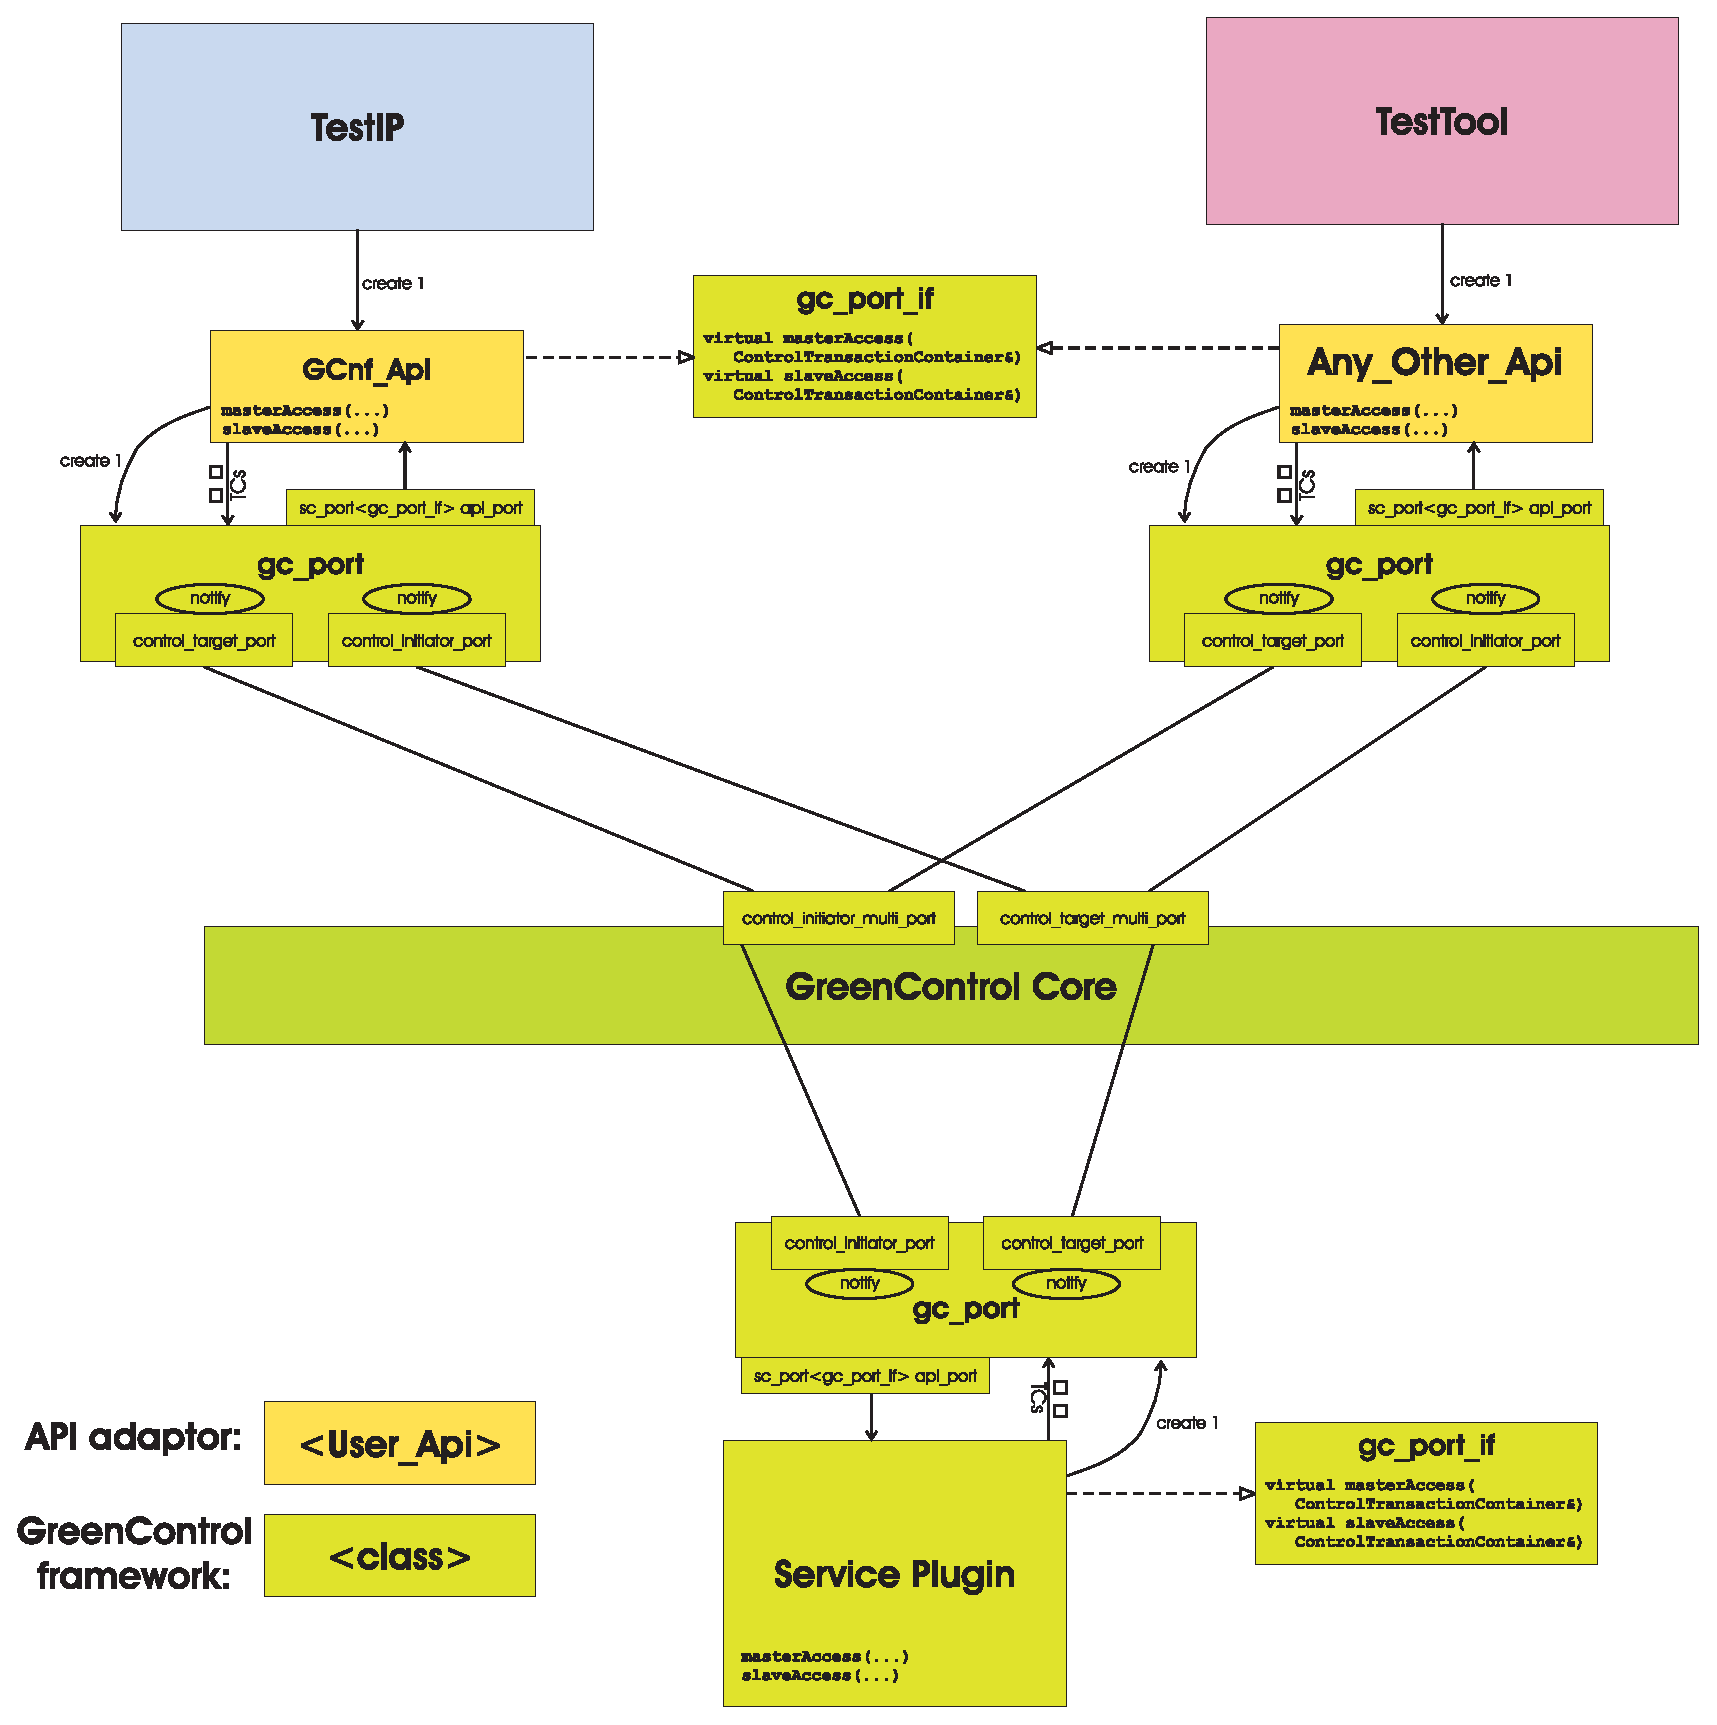
\includegraphics[width=\textwidth]{GreenControlImpl2.eps}
	} 
	\caption{This image shows how the GreenControl implementation is realized. }
	\label{fig:GreenControlImpl}
\end{figure}


%%%%%%%%%%%%%%%%%%%%%%%%%%%%%%%
\section{Namespace gs::ctr and naming conventions}
\label{GreenControlNamespaceAndConventions}
This framework is placed inside the namespace {\sffamily gs::ctr} which is a sub namespace of the GreenSocs namespace {\sffamily gs}. All \GreenControl classes are placed in this namespace.

\Note{Compatibility Note}{Namespace compativility to release 0.2}{
	To be compatible to the old namespaces (tlm::gc, tlm::gc::config) the header
	file \Datei{greencontrol/namespace\_compatibility.h} can be included!
}

For the correct namespace of the classes used in this document please
refer to the doxygen generated API reference.

The classes that are visible to the user have the prefix \lstinline|gc| or \lstinline|GC|.

The \GreenControl framework, and this  documentation make use of some abbreviations:
\begin{itemize}
	\item \emph{GC} means \emph{GreenControl},
\end{itemize}


%%%%%%%%%%%%%%%%%%%%%%%%%%%%%%%
\section{Files}
\label{GreenControlFiles}
The GreenSocs package \emph{greencontrol} contains the framework files.

The framework is organized in subdirectories:
\begin{itemize}

  \item \Verzeichnis{greencontrol}:\newline
  	Main user include files for the Core and services.

  \item \Verzeichnis{greencontrol/core}:\newline
  	\GreenControl Core with all classes needed by the user to create the core and needed by the plugins and APIs for connection.

  \item \Verzeichnis{greencontrol/\textless servicename\textgreater}: \newline
  	For each service which can be added to the framework, a subdirectory is created which contains 
    \begin{itemize}
      \item \Verzeichnis{plugin}: a plugin directory and 
      \item \Verzeichnis{apis}: an API's directory
    \end{itemize}
    Each service should provide a single include header file in the \Verzeichnis{greencontrol} folder. The file should include the basic classes needed for the service.

  \item \Verzeichnis{greencontrol/docs/\textless servicename\textgreater}: \newline
  	Documentation directory with one subdirectory for each service.

  \item \Verzeichnis{greencontrol/examples}: \newline
  	Examples

\end{itemize}

\noindent
\begin{minipage}{\textwidth}
\begin{tabularx}{\textwidth}{|l|X|}
	\cline{1-1}\cline{2-2}\multicolumn{2}{|l|}{ {\bf greencontrol}    }\\ 
	\cline{1-1}\cline{2-2} core.h    &  The include file for the user. \\ 
	\cline{1-1}\cline{2-2}\multicolumn{2}{|l|}{  {\bf greencontrol/core}    }\\ 
	\cline{1-1}\cline{2-2} controladdressmap.h    &  Used by the Core: class \lstinline|ControlAddressMap| to provide a map for address resolution (name to port number in multi port).   \\ 
	\cline{1-1}\cline{2-2} controlports.h    &  Ports to transport transaction containers: \mbox{\lstinline|control_target_port|,} \mbox{\lstinline|control_target_multi_port|,} \mbox{\lstinline|control_initiator_port|}, \mbox{\lstinline|control_initiator_multi_port|.}   \\ 
	\cline{1-1}\cline{2-2} gc\_core.h    &  \GreenControl Core which routes the ControlTransactionContainer to the target. Main file which has to be included by the top level (testbench). \\ 
	\cline{1-1}\cline{2-2} gc\_globals.h    &  Global settings for \GreenControl, needed by all other header files. \\ 
	\cline{1-1}\cline{2-2} gc\_port\_if.h    &  Interface with the virtual methods \lstinline|masterAccess(ControlTransactionContainer\&)| and \lstinline|slaveAccess(ControlTransactionContainer\&)|. Must be implemented by APIs which want to use the gc\_port. These methods are called when a transaction arrives at the initiator or target port.   \\ 
	\cline{1-1}\cline{2-2} gc\_port.h    &  The class \lstinline|gc_port| is the port to the \GreenControl Core. It has a sc\_port \lstinline|api_port| which has to be bound by the API (either \lstinline|GCnf_Api| or a User API) to serve incoming transactions. Outgoing transactions can be sent with notify(transaction) in its target and master ports.   \\ 
	\cline{1-1}\cline{2-2} gc\_transaction.h    &  Holds the transaction container and the phases; classes/typedefs: \lstinline|ControlTransaction|, \lstinline|ControlTransactionHandle|, \lstinline|ControlPhase|,  \lstinline|ControlPhaseHandle|, \lstinline|ControlTransactionContainer|   \\ % TODO: remove phases?
	\cline{1-1}\cline{2-2} gcexception.h    &  \GreenControl-wide exception base class with special derived exception classes (e.g. command line parser exception).   \\ 
	\cline{1-1}\cline{2-2} gcnf\_api\_if.h    &  Interface \lstinline|gcnf_api_if|: Allows the \GreenControl Core to control the initialize-mode for initial configuration.   \\ 
	\cline{1-1}\cline{2-2} gscontrol.h    &  Information file. Not to be included.  \\ 
	\cline{1-1}\cline{2-2} helpfunctions.h    &  Some helping functions which are used by various classes.  \\ 
	\hline
\end{tabularx}
\end{minipage}

\vspace{1 cm}

\noindent
\begin{minipage}{\textwidth}
\begin{tabularx}{\textwidth}{|l|X|}
	\cline{1-1}\cline{2-2}\multicolumn{2}{|l|}{  {\bf greencontrol/core/transport}    }\\ 
	\cline{1-1}\cline{2-2} *    &  These files represent the communication structure which is based on the \GreenBus project using TLM-2.0 concepts (not the OSCI TLM-2.0 implementation!).  \\ 
	\hline
\end{tabularx}
\end{minipage}

\vspace{1 cm}


%%%%%%%%%%%%%%%%%%%%%%%%%%%%%%%
\section{Communication}

The \GreenControl Core originally is based on \GreenBus and adopts its concepts. To allow even greater performance and maintainability than \GreenBus some well-chosen elements have been copied to the \GreenControl framework (directory \Verzeichnis{greencontrol/core/transport}). This also removes the dependence on the \GreenBus package and allows GreenControl and its plugins being used within the \GreenBus core.

\subsection{Port binding}
\label{commPortBinding}
\begin{itemize}
	\item All APIs and API adapters get their ports \lstinline|control_initiator_port| and \lstinline|control_target_port| automatically by using (instantiating) \lstinline|gc_port|. 

	\item As a result of this instantiation the Core can identify these APIs and its ports when going through the object hierarchy. The Core can bind the ports automatically to the multi ports of the Core. This automatically binding is done either by the Core during before\_end\_of\_elaboration or by each \lstinline|gc_port| after port construction for immediate binding (call of \lstinline|process_ports()|). \newline The Core goes through the sim context hierarchy and searches for instances of the \lstinline|control_xx_port|s and saves pointers to them into a list (if not yet in it). Afterwards these ports are automatically bound to the multi ports of the Core (if not yet done). Hence the user need not bind the ports themselves. 
	
	\item The Core can identify already bounded ports with the
	call \lstinline|is_Bound()|, so it is does not bind ports
	twice, e.g. if each port does immediate binding.
	
	\item The constructors of the control ports ask for special information: 
	\begin{itemize}
		\item APIs and plugins have to specify their supported control service. 
		\item Plugins have to set a bool to true to show that a plugin is connected to serve all transactions to its supported service. 
		\item APIs and plugins have to specify their target address (type \lstinline|cport_address_type|) which has to be set to the pointer address of their \lstinline|gc_port|. 
		\item APIs and plugins submit a human readable unique name which is used for debug and maybe future use. 
		\item These variables are read by the Core when building the address map (see section \ref{commAddressing}). 
	\end{itemize}

\end{itemize}


\subsection{Addressing}
\label{commAddressing}
The \GreenControl Core routes the transaction containers with the two fields "Service" and "Target". The target field is the address (\lstinline|gc_port|'s pointer address) of the API or plugin where the transaction should be delivered. The service field specifies the service which is used for categorization (for analyzing the communication) and is used for routing:  

If the sender does not know the correct address of the plugin which is responsible for the service (normal case!), the sender may leave the target field blank (\lstinline|0|) and only set the service field. The router knows which plugin belongs to which service (because of the constructor parameters of the ports, see section \ref{commPortBinding}) and routes the transaction to the (only) plugin supporting that service. 

The plugin has to know the address of the API it wants to reach. That is no problem because each API first sends a transaction to the plugin (e.g. parameter add, set or observer registration) and the plugin stores the MasterID (which can be found in the transaction container) as target address for that API/module). 

The target address allows a user module to use multiple (different) APIs for one service (e.g. it uses scml parameters and GCnf parameters).  



\subsection{Port usage in the APIs}
This is about how to use the ports inside an implementation of an User API adapter. 

The interface \lstinline|gcnf_api_if| waits for two methods: 

\begin{itemize}
\item \lstinline|masterAccess(ControlTransactionContainer&)| and 

\item \lstinline|slaveAccess(ControlTransactionContainer&)| 


\end{itemize}
These methods are called by the port (the included payload event
queue, peq) instead of generating a \lstinline|default_event()|. This
call is faster than an event which has to be scheduled by the kernel
{\em and may be used during elaboration}. So each transaction that
arrives results in a call to one of these methods. \lstinline|masterAccess| is called when a master accesses the target port, \lstinline|slaveAccess| is called when a slave accesses the master port. 

The ports \lstinline|control_initiator_port| and \lstinline|control_target_port| are located in the \lstinline|gc_port| and can be accessed through the variables \lstinline|init_port| and \lstinline|target_port|. 


%\begin{landscape}
\begin{table}[htbp] 
\begin{center}
\begin{sideways}
\begin{tabularx}{23cm}{|p{2.3cm}|p{2.4cm}|p{3cm}|X|X|X|}
	\cline{1-1}\cline{2-2}\cline{3-3}\cline{4-4}\cline{5-5}\cline{6-6} {\em Field name}     &  {\em Member name}    &  {\em Data type}    &  {\em Example 1}    &  {\em Example 2}    &  {\em Explanation}   \\ 
	\cline{1-1}\cline{2-2}\cline{3-3}\cline{4-4}\cline{5-5}\cline{6-6} {\bf {\textsf Service}}      &  mService           &  ControlService (enum)    &  \lstinline|CONFIG_SERVICE|    &     &  Service specification; used for routing to the correct plugin and analysis  \\ 
	\cline{1-1}\cline{2-2}\cline{3-3}\cline{4-4}\cline{5-5}\cline{6-6} {\bf {\textsf Target}}, \mbox{\bf {\textsf Address}}     &  mTarget    &  cport\_address\_type (void*)    &  \lstinline|3215719780|    &  \lstinline|3215759780|    &  Routing target (address of API or plugin) where the Core should route the transaction to   \\ 
	\cline{1-1}\cline{2-2}\cline{3-3}\cline{4-4}\cline{5-5}\cline{6-6} {\bf {\textsf Command}}      &  mCmd    &  unsigned int (for specialized enumerations)    &  \lstinline|CMD_SET_PARAM|    &  \lstinline|CMD_GET_PARAM_LIST|    &  Command the target should execute, available commands are dependent on the service. \\ 
	\cline{1-1}\cline{2-2}\cline{3-3}\cline{4-4}\cline{5-5}\cline{6-6} {\bf {\textsf AnyPointer}}      &  mAnyPointer    &  void*  &    &    & Field for any type of pointer, initiator and target must know the type and do casts.\\ 
	\cline{1-1}\cline{2-2}\cline{3-3}\cline{4-4}\cline{5-5}\cline{6-6} {\bf {\textsf AnyPointer2}}      &  mAnyPointer2    &  void*  &    &    & Another field for any type of pointer. \\ 
	\cline{1-1}\cline{2-2}\cline{3-3}\cline{4-4}\cline{5-5}\cline{6-6} {\bf {\textsf AnyUint}}      &  mAnyUint    &  unsigned int  &    &    & Field for any type of unsigned int information. \\ 
	\cline{1-1}\cline{2-2}\cline{3-3}\cline{4-4}\cline{5-5}\cline{6-6} {\bf {\textsf Specifier}}    &  mSpecifier    &  ControlSpecifier (string)    &  \lstinline|jpeg.compressionParam1|    &  \lstinline|mymodule.submodule.param2|    &  The affected object; different concerning to the command   \\ 
	\cline{1-1}\cline{2-2}\cline{3-3}\cline{4-4}\cline{5-5}\cline{6-6} {\bf {\textsf Value}}        &  mValue    &  ControlValue (string)    &  \lstinline|"42"|    &  \lstinline|"myTestValue"|    &  Value; different concerning to the command   \\ 
	\cline{1-1}\cline{2-2}\cline{3-3}\cline{4-4}\cline{5-5}\cline{6-6} {\bf {\textsf MasterID}}     &  mID    &  cport\_address\_type (void*)    &  \lstinline|3213638188|    &     &  Address of the sender API or plugin. Automatically set by port.   \\ 
	\cline{1-1}\cline{2-2}\cline{3-3}\cline{4-4}\cline{5-5}\cline{6-6} {\bf {\textsf Error}}        &  mError    &  unsigned int    &  \lstinline|0|    &  \lstinline|1|    &  Error code for response (0=no error)   \\ 
	\hline
\end{tabularx}
\end{sideways}
\end{center}
\caption{Fields of the Transaction Container. }
\label{tbl:TransactionContainer}
\end{table}
%\end{landscape}

\subsection{Transaction Container}

The transaction container consists of various fields (see table \ref{tbl:TransactionContainer} on page \pageref{tbl:TransactionContainer}).

The command field is kept general as an unsigned integer. Since the
transaction object \lstinline|ControlTransaction| could be used by
various services this field is dependent on the  specific service
being used. The APIs and plugins should use an enumeration which is specialized for their service.

Not all fields are necessarily used by each service. Since we have a pool of existing transaction objects and not all fields are reseted each time being reused there is no performance issue having more fields than needed.

The sender of a transaction {\em must ensure} that {\em all} fields that are processed by the receiver are set or reseted because transactions are taken out of the pool and may contain not reseted fields! The only fields that are reseted by default are the \textsf{Error} field and the \textsf{Service} field. 

See \GreenConfig User's Guide for the available commands for the configuration service and how to add new commands for that service.


\subsection{Phases}
% TODO: Phase entfernen, blockende Kommunikation???
The communication between two members is done with several phases (as
it is done in \GreenBus generally). As the communication inside the SystemC world is reliable we need no handshake phases. Accordingly we need two phases for a request with an answer: 

\begin{itemize}
\item \lstinline|REQUEST| 
\item \lstinline|RESPONSE|. 
\end{itemize}

The Request phase sends the request transaction container to the
target, the target adds the response to the transaction container and
sends it during the Response phase back to the sender. Because there
is an Error field which has to be sent back to the sender, the
Response phase is even needed when there is no other data to be sent
back.


%%%%%%%%%%%%%%%%%%%%%%%%%%%%%%%
\section{Order for constructing GreenControl elements}
\label{OrderConstructionElements}
The \GreenControl framework requires the a strict constructing order. It is recommended to instantiate the elements manually observe the following rules. Alternatively the automatic mechanism described afterwards can be used if there is no way to ensure that the \GreenControl elements are instantiated before any code accessing the services, e.g. in a tool environment.

\begin{itemize}

  \item Before any other \GreenControl elements may be instantiated or used, the singleton \emph{Core} is needed.
\begin{lstlisting}
gs::ctr::GC_Core   core("ControlCore");
\end{lstlisting}
Alternatively use the following static function call which will create (at first call) and return the singleton (each call):
\begin{lstlisting}
gs::ctr::GC_Core::get_instance();
\end{lstlisting}

  \item Afterwards other \GreenControl elements may be instantiated, beginning with the plugins. For example the Configuration Service within the namespace \lstinline|gs::cnf| is the next one to instantiate:
\begin{lstlisting}
gs::cnf::ConfigPlugin   configPlugin("ConfigPlugin", database);
\end{lstlisting}
See the related documentation for the recommended and possible ways of creating the service plugins.

  \item The plugin instantiations may be followed by any User APIs and modules (containing User APIs). 
\end{itemize}

The construction order for plugins, APIs and modules is not fixed. Depending on the application different orders may be useful. In general it will be reasonable to instantiate all plugins prior to modules which make use of them. If a user module tries to make use of a not existing service plugin during its construction the routing of the transaction will fail and result in a routing error.

\subsection{Alternative automatic construction}
Alternatively to the manual Core instantiation, you can rely on its automatic creation. During the first creation of a \lstinline|gc_port| the Core will be created by the static get instance function being called by the port constructor. Typically this should be the case when creating the first service plugin, e.g. the configuration plugin.

See the related documentation for possible automatic instantiations of the plugins.

%%%%%%%%%%%%%%%%%%%%%%%%%%%%%%%
\section{Command line options/switches}
Some API Tools may need to parse command line options and switches, e.g. config file parser to get the filename (see \GreenConfig documentation), config command line parser to get parameter values etc.

To get a variable framework where these APIs and tools can be added and removed very easily we have to use a general approach for parsing the command line: 

To achieve highly modularity each API tool, which needs to parse the command line, gets the whole command line arguments like they are submitted to the \lstinline|main| method. The parser then only processes the options and switches which are supported by that parser and ignores the other ones. The parsers must not change the \lstinline|argc| value and the \lstinline|argv| array because all parser should get the original values. The parser should work on a copy of the argument array: if e.g. the command \lstinline|getopt| or \lstinline|getopt_long| is used, a copy of \lstinline|argv| has to be used because these methods change the arrays during processing. 

\begin{itemize}
	\item It is essential to {\em make sure that each option or switch is used only once in the entire framework}. 

	\item The parsers may make use of (and throw or throw and catch) the exception class \lstinline|CommandLineException|. 

	\item All parsers should parse the '--help' and '-h' switch to print out usage information. 
	
	\item None of these parsers is allowed to make use of non-option and non-switch arguments because they are printed out by the core to allow a minimal user information on wrong used
arguments: The switches and options are parsed by the concerned parser and remaining elements (due to wrong placed spaces etc.) should be printed out as failures. 
\end{itemize}


%%%%%%%%%%%%%%%%%%%%%%%%%%%%%%%
\section{Initialize-mode}
\label{InitializeMode}
The \GreenControl framework provides the {\em initialize-mode} which can be used by plugins and APIs to differ between elaboration and runtime without the need to derive from SystemC modules.

\GreenControl may be used immediately after construction (even before simulation runtime) because we use immediate communication without events in the underlying \GreenBus framework.

To give the APIs the opportunity to check if the time is during initialize-mode there are callbacks:

If the APIs had to override the kernel callback functions to make their elaboration configuration
they would be forced to be SystemC modules. But we don't want them to be modules. So we have our own
interface (\lstinline|gcnf_api_if|) which has to be implemented by each API which wants to use the
initialize-mode. But even if an API does not need the initialize-mode each API has to implement this interface so that they can also be identified as interfaces for other issues (e.g. routing). The interface contains the callback functions
\lstinline|start_initial_configuration| and \lstinline|end_initialize_mode|. Both functions are called by the Core while it processes the start\_of\_simulation callback. The first callback (\lstinline|start_initial_configuration|) may be used for initial configuration which was not yet done at construction time. The latter (\lstinline|end_initialize_mode|) shows the end of initialize-mode. From that point on the framework may be used in {\em runtime-mode}. With the help of these callbacks plugins and APIs can identify simulation runtime. Before and during the initialize-mode {\em no} events, notifies, time (even SC\_ZERO\_TIME) are allowed.

An example how to use the initialize-mode callbacks can be seen in the \GreenConfig API.


%%%%%%%%%%%%%%%%%%%%%%%%%%%%%%%
\section{Miscellaneous}
\label{GCMiscellaneous}

\subsection{SystemC 2.1}
When using \GreenControl with SystemC 2.1 there may be warnings like the one below. For OSCI SystemC 2.1v1 there is a workaround. Within other SystemC implementations these warnings can be presumably ignored. \newline
\begin{quote}
{\sffamily Warning: (W505) object already exists: fec. Latter declaration will be renamed to fec\_24 \newline
In file: ../../../../src/sysc/kernel/sc\_object.cpp:187} \newline
\end{quote}

\Note{Implementation Note}{Background SystemC 2.1 warning}{
  When the payload event queue creates a SC\_METHOD during end\_of\_elaboration, all these methods get the same name (``fec''). Especially in SystemC 2.1 all these methods are situated within the {\em same} hierarchy level (toplevel). Accordingly SystemC warns that the objects are renamed. The workaround uses OSCI code which is behind the SC\_METHOD macro, accordingly this is no standard and maybe only works with OSCI SystemC.
}



\end{document}
